\chapter{Umsetzung}

\section{Vorgehensmodell}

\subsection{Metriken Identifizieren}

\subsubsection{\ac{GQM}}

Um eine Vorauswahl an Metriken treffen zu können, wurden alle bisherigen Retrospektiven (es waren genau 15) analysiert und eine Topliste von Schlagwörtern der folgenden Fragestellungen aus den Retrospektiven erstellt:
\begin{enumerate}
    \item Welche guten Entscheidungen haben wir getroffen?
    \item Was haben wir gelernt?
    \item Was können wir besser machen?
    \item Was nervt uns noch immer?
\end{enumerate}

Dazu wurden die Ergebnisse in eine ElasticSearch Datenbank gespeichert und über eine sogenannte Terms Aggregation die wichtigsten Schlagwörter analysiert.
Bei der Indizierung werden die Wörter normalisiert, deshalb die teilweise andere Schreibweise (zum Beispiel wird aus Issue der Term issu).
Die Ergebnisse in Anhang~\ref{appendix:retros} sind für die einzelnen Punkte wie folgt interpretierbar:

\begin{description}
    \item[Welche guten Entscheidungen haben wir getroffen?] \hfill
    \begin{itemize}[noitemsep]
      \item Die ersten fünf Wörter lassen darauf schließen, dass das Team gut zusammenarbeitet, speziell bei der Wissensverteilung: Transparenz, Onboarding von neuen Themen und Pair-Programming.
      \item Ebenfalls lässt sich aus den weiteren Begriffen schließen, dass viel Wert auf Reviews, Daily und die Arbeitsweise an sich gelegt wird.
    \end{itemize}
    \item[Was haben wir gelernt?] \hfill
    \begin{itemize}[noitemsep]
      \item Auch hier spiegelt sich der Daten- und Kommunikationsfluss im Team wider.
      \item Die vielen Scrum Schlagwörter zeigen, dass die Retrospektiven richtig genutzt wurden, um den Prozess zu verbessern.
    \end{itemize}
    \item[Was können wir besser machen?] \hfill
    \begin{itemize}[noitemsep]
      \item Auch hier zeugen die Scrum Schlagwörter wieder von einer Prozessverbesserung und einem selbstreflektiven Verhalten.
      \item Die Dokumentation scheint teilweise noch ein Problem zu sein, diese kommt gleich zweimal vor.
      \item Issues scheinen teilweise nicht optimal zu sein. Da könnte das Schlagwort ``groß'' dazu passen.
      \item ``backlog'', ``blocked'' und ``àblauf'' lassen auf Probleme im Arbeitsablauf schließen.
    \end{itemize}
    \item[Was nervt uns noch immer?] \hfill
    \begin{itemize}[noitemsep]
      \item Hier lassen die Schlagwörter ``updat'', ``erreichbar'', ``infrastruktur'', ``jenkin'', ``test'' und ``umgebung'' auf ein Infrastruktur Problem schließen, welches das Team womöglich ausbremst.
      \item Die Schlagwörter ``lang'', ``groß'' und ``klar'' lassen auf Probleme mit Anforderungen beziehungsweise Stories schließen.
      \item ``apis'', ``dba'', ``laut'' und ``iso'' sind wahrscheinlich äußere Einflüsse, die bei der täglichen Arbeit stören.
    \end{itemize}
  \end{description}

Aus diesen Ergebnissen Lassen sich die \ac{GQM}-Modelle in Tabelle~\ref{tab:gqm-distraction},~\ref{tab:gqm-process} und~\ref{tab:gqm-issues} ableiten.

\begin{table}[H]
    \centering
    \begin{tabular}{llr}
    GOAL     & \begin{tabular}[c]{@{}l@{}}Absicht\\ Problem\\ Ressource\\ Sichtweise\end{tabular} & \begin{tabular}[c]{@{}l@{}}Verringerung\\ der Ablenkung\\ von Entwicklern\\ aus Sicht des Scrum Masters.\end{tabular} \\ \midrule
    QUESTION & \multicolumn{2}{l}{Wie viele Aufgaben erledigt das Team pro Sprint?} \\
    METRIC   & \multicolumn{2}{l}{Aufgaben-Volumen pro Sprint} \\ \midrule
    QUESTION & \multicolumn{2}{l}{Wie viele Aufgaben werden jeden Tag erledigt?} \\
    METRIC   & \multicolumn{2}{l}{\begin{tabular}[c]{@{}l@{}}erledigte Aufgaben pro Tag\\ Burn-down pro Tag\end{tabular}} \\ \midrule
    QUESTION & \multicolumn{2}{l}{Welche Tags haben als ``schlecht'' bewertete Aufgaben?} \\
    METRIC   & \multicolumn{2}{l}{\begin{tabular}[c]{@{}l@{}}Tags der Aufgaben, \\ um ``schlecht'' bewertete besser analysieren zu können\end{tabular}}
    \end{tabular}
    \caption{GQM\mbox{-}Modell \mbox{-} Ablenkung der Entwickler}\label{tab:gqm-distraction}
\end{table}

\begin{table}[H]
    \centering
    \begin{tabular}{llr}
    GOAL     & \begin{tabular}[c]{@{}l@{}}Absicht\\ Problem\\ Prozess\\ Sichtweise\end{tabular} & \begin{tabular}[c]{@{}l@{}}Optimierung\\ des Durchlaufes\\ im Entwicklungsprozess\\ aus Sicht des Scrum Teams.\end{tabular} \\ \midrule
    QUESTION & \multicolumn{2}{l}{Gibt es irgendwelche Engpässe im Prozess?} \\ 
    METRIC   & \multicolumn{2}{l}{Cumulative Flow} \\ \midrule
    QUESTION & \multicolumn{2}{l}{Wie lange dauert der Durchlauf einer Aufgabe?} \\
    METRIC   & \multicolumn{2}{l}{Lead Time}
    \end{tabular}
    \caption{GQM\mbox{-}Modell \mbox{-} Schwachstellen im Prozess}\label{tab:gqm-process}
\end{table}

\begin{table}[H]
    \centering
    \begin{tabular}{llr}
    GOAL     & \begin{tabular}[c]{@{}l@{}}Absicht\\ Problem\\ Ressource\\ Sichtweise\end{tabular} & \begin{tabular}[c]{@{}l@{}}Optimierung\\ der Aufgabengröße\\ im Backlog\\ aus Sicht des Product Owners.\end{tabular} \\ \midrule
    QUESTION & \multicolumn{2}{l}{Wie groß ist die Aufgabengröße im Durchschnitt?} \\
    METRIC   & \multicolumn{2}{l}{erledigte Story-Points / Aufgaben-Volumen} \\ \midrule
    QUESTION & \multicolumn{2}{l}{Wie lange dauert der Durchlauf einer Aufgabe?} \\
    METRIC   & \multicolumn{2}{l}{Lead-Time} \\ \midrule
    QUESTION & \multicolumn{2}{l}{Wie viele Aufgaben gehen im Entwicklungsprozess rückwärts?} \\
    METRIC   & \multicolumn{2}{l}{Aufgaben-Rückfälligkeit}
    \end{tabular}
    \caption{GQM\mbox{-}Modell \mbox{-} Aufgabengröße}\label{tab:gqm-issues}
\end{table}

\subsubsection{Umfrage im Team}

Zusätzlich zu der Analyse der Retrospektiven wurden dem Team Metriken und die Fragen, die damit beantwortet werden können, in Form einer Umfrage vorgestellt.
Die einzelnen Metriken wurden von den Teammitgliedern nach Wichtigkeit mit einer Skala von 1 bis 10 bewertet.
Anhang~\ref{appendix:questions} zeigt die Umfrage, wie sie den Teammitgliedern vorgelegt wurde und Anhang~\ref{appendix:answers} die dazugehörigen Antworten.
Die Ergebnisse wurden nach ihrem Druchschnittwert sortiert und die 10 als am wichtigsten bewerteten Metriken sind:

\begin{itemize}[noitemsep]
    \item \textbf{Burn Down (9,00)} \mbox{-} Erfüllt das Team seine Commitments? Plant das Team seine Arbeit realistisch?
    \item \textbf{Velocity (9,00)} \mbox{-} Wie konsistent arbeitet das Team?
    \item \textbf{Aufgaben-Volumen (8,57)} \mbox{-} Wie viel ungeplante Arbeit kam zum Sprint dazu? Wie groß ist die durchschnittliche Aufgabe? Gibt es Ausreißer?
    \item \textbf{Cumulative Flow (8,29)} \mbox{-} Gibt es Engpässe oder Schwachstellen im Prozess? Müssen gewisse Abläufe im Prozess optimiert werden?
    \item \textbf{Lead Time (8,14)} \mbox{-} Wie schnell können Aufgaben vom Team erledigt werden? Wie lange dauert die Umsetzung eines neuen Features?
    \item \textbf{Stresstests oder Benchmarking (7,86)} \mbox{-} Ist das Produkt auch noch unter Last verwendbar? Wie verändert sich die Leistung über die Zeit?
    \item \textbf{Code Coverage (7,71)} \mbox{-} Gibt es Module, die nicht oder schlecht getestet sind? Wie sieht die Entwicklung der Testabdeckung über die Zeit aus?
    \item \textbf{Bug Counts (7,57)} \mbox{-} Wie viele Fehler werden vom Team im Entwicklungsprozess übersehen? Wie viel ungeplante Arbeit kam zum Sprint dazu?
    \item \textbf{Aufgaben-Rückfälligkeit (7,57)} \mbox{-} Wie viele Aufgaben werden wieder in einen vorhergehenden Status gesetzt? Gibt es Probleme beim Verständnis der Aufgaben? Wie klar sind die Erwartungen des Teams an eine abgeschlossene Änderung (DoD)?
    \item \textbf{Bug-Erzeugungsrate (7,43)} \mbox{-} Wie viele Fehler wurden zu einem bestimmten Zeitpunkt erzeugt?
\end{itemize}

Zusätzlich wurde in den offenen Fragen am Ende zwiemal gefordert, dass die Flüchtigkeit von Anforderungen Sichtbar wird. 
Dies kann zum einen durch die oben genannte Aufgaben-Rückfälligkeit und andererseits durch folgende Metrik abgebildet werden:

\begin{itemize}[noitemsep]
    \item \textbf{Anforderungen-Flüchtigkeit} \mbox{-} Wie oft wurde die Anforderung der Aufgabe angepasst?
\end{itemize}

\section{Software}

Technologien, Plattform, etc.

\subsection{Architektur}

Abbildung~\ref{fig:position_architecture} zeigt die Position und Abbildung~\ref{fig:overview_architecture} die grobe Architektur der Software (Agile Metrics).
Die Software bildet eine Schnittstelle zwischen den einzelnen Systemen des Entwicklungsprozesses und dem System zur Darstellung der Metriken (in diesem Fall ElasticSearch und Kibana).

\begin{savenotes}
    \begin{figure}[H] 
        \centering
            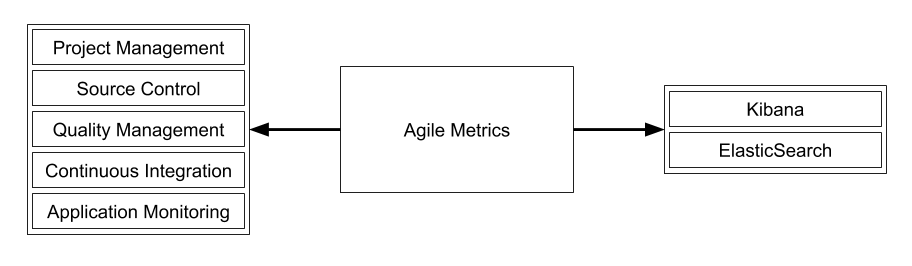
\includegraphics[width=0.8\textwidth]{img/position-overview.png}
        \caption{Position der Software}\label{fig:position_architecture}
    \end{figure}
\end{savenotes}

\begin{savenotes}
    \begin{figure}[H] 
        \centering
            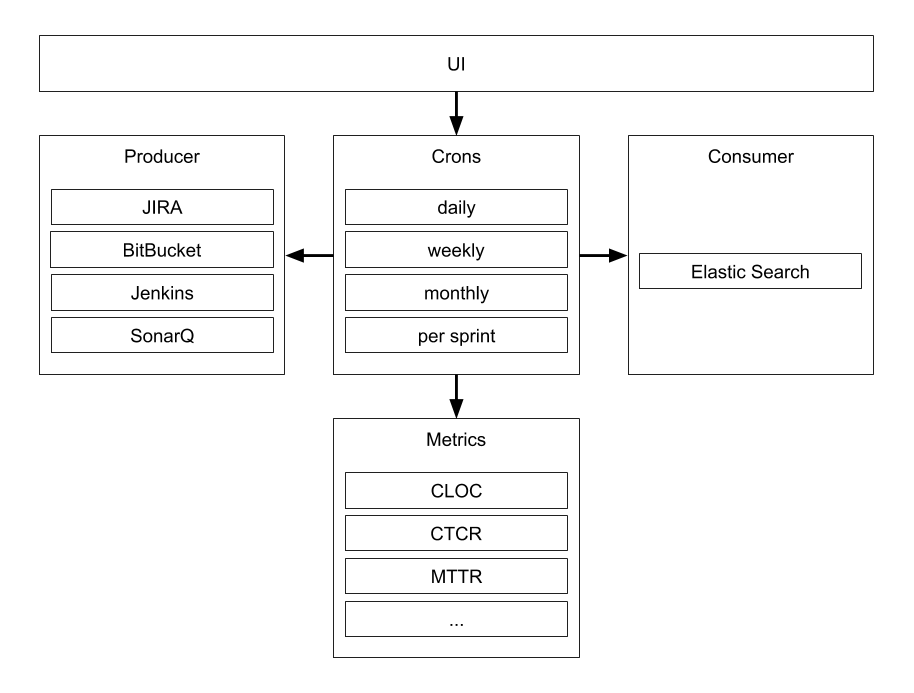
\includegraphics[width=0.8\textwidth]{img/architecture-overview.png}
        \caption{Übersicht der Software-Architektur}\label{fig:overview_architecture}
    \end{figure}
\end{savenotes}

\begin{description}
    \item[UI] \hfill \\ Bietet eine grafische Benutzeroberfläche zur Konfiguration.
    \item[Producer] \hfill \\ Sind Schnittstellen zu allen Systemen, die Messdaten erzeugen.
    \item[Crons] \hfill \\ Zeitsteuerung der Messdaten-Abfrage (z.B. täglich oder pro Sprint).
    \item[Metrics] \hfill \\ Hier können aus Messdaten direkt Metriken erstellt werden.
    \item[Consumer] \hfill \\ Sind Schnittstellen zu allen Systemen, die Messdaten und Metriken konsumieren.
\end{description}
